\chapter{Implementación}
Durante la implementación, se ha seguido la planificación y metodologías
anteriormente descritas, dividiendo el proyecto en tareas más pequeñas y
manejables, para que se puedan realizar en un periodo de tiempo razonable.

Al seguir la prioridad de las tareas, se realizan primero las tareas más
críticas, como la creación de la infraestructura y la ingesta de las fuentes
esenciales, y se dejan para más adelante tareas como la visualización para
clientes externos o fuentes menos críticas y más complejas, como las APIs de
terceros o el \textit{web scraping}.


\section{Despliegue local}\label{sec:impl_local}
Para arrancar el desarrollo del proyecto, se decide construir una versión
local del sistema, que permita trabajar en un entorno controlado y sin
dependencias externas para comprobar su correcto funcionamiento y establecer
las bases de configuración y del posterior despliegue en la nube.

Puesto que se ha decidido utilizar Docker para la gestión de contenedores, se
ha creado un archivo \texttt{docker-compose.yml} que define los servicios
necesarios para el proyecto, es decir, \textit{Kafka}, \textit{Zookeeper},
\textit{Elasticsearch}, \textit{Kibana} y \textit{Logstash}, ignorando por
el momento la ingesta de datos y la escalabilidad del sistema.

Para la configuración de los servicios, se ha creado un archivo \texttt{.env}
que define las variables de entorno necesarias para el correcto funcionamiento
de los servicios, como las contraseñas o la versión del \textit{stack}.

Durante el arranque de los contenedores, se ejecuta un script de inicialización
que se encarga de crear las credenciales y los usuarios necesarios para el
funcionamiento de los servicios. Estas credenciales son necesarias ya que los
contenedores funcionan mediante tráfico HTTPS.

Los contenedores cuentan con comprobaciones de salud (o \textit{health-checks})
básicas para asegurar que los servicios se han arrancado correctamente y están
funcionando.

Una vez arrancados los contenedores mediante el comando
\texttt{docker compose up}, se puede acceder a los servicios a través de la
dirección local \texttt{localhost}. En el caso de Kibana, se puede acceder a
la interfaz de usuario mediante la dirección \texttt{localhost:5601}. En el
caso de Elasticsearch, se pueden hacer peticiones HTTPS a través de la dirección
\texttt{localhost:9200}. Para Kafka, Zookeeper y Logstash, se pueden hacer
peticiones a través de las direcciones \texttt{localhost:9092},
\texttt{localhost:2181} y \texttt{localhost:9600}, respectivamente.

\begin{figure}[H]
	\centering
	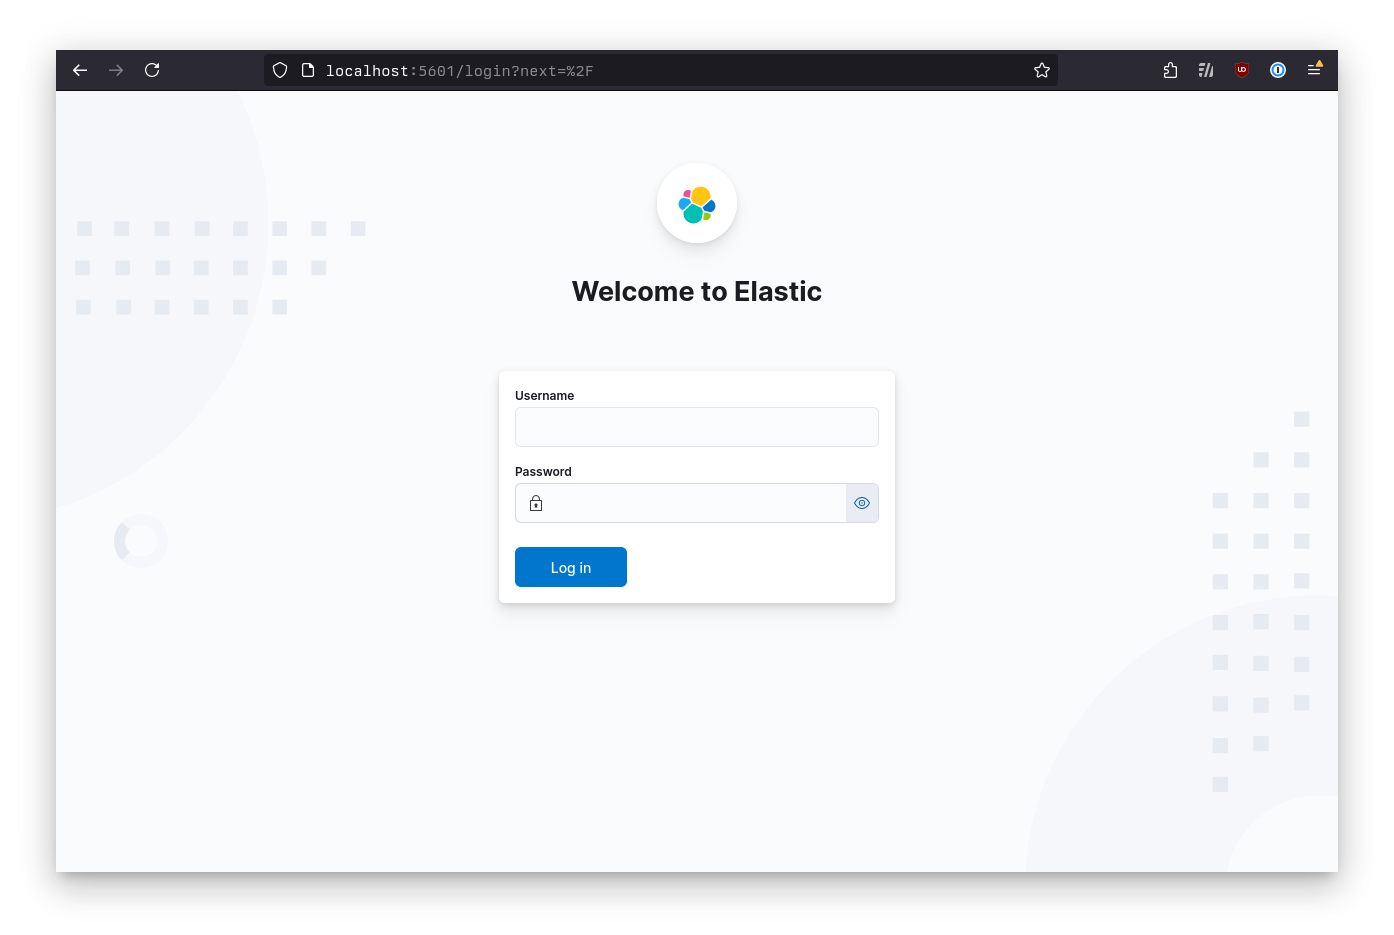
\includegraphics[width=\textwidth]{impl/local1.png}
	\caption{Inicio de sesión en Kibana}
	\label{fig:kibana_login}
\end{figure}

Una vez en la pantalla de inicio de sesión, se puede acceder con las credenciales
definidas en el archivo \texttt{.env} para el usuario \texttt{elastic}.

\begin{figure}[H]
	\centering
	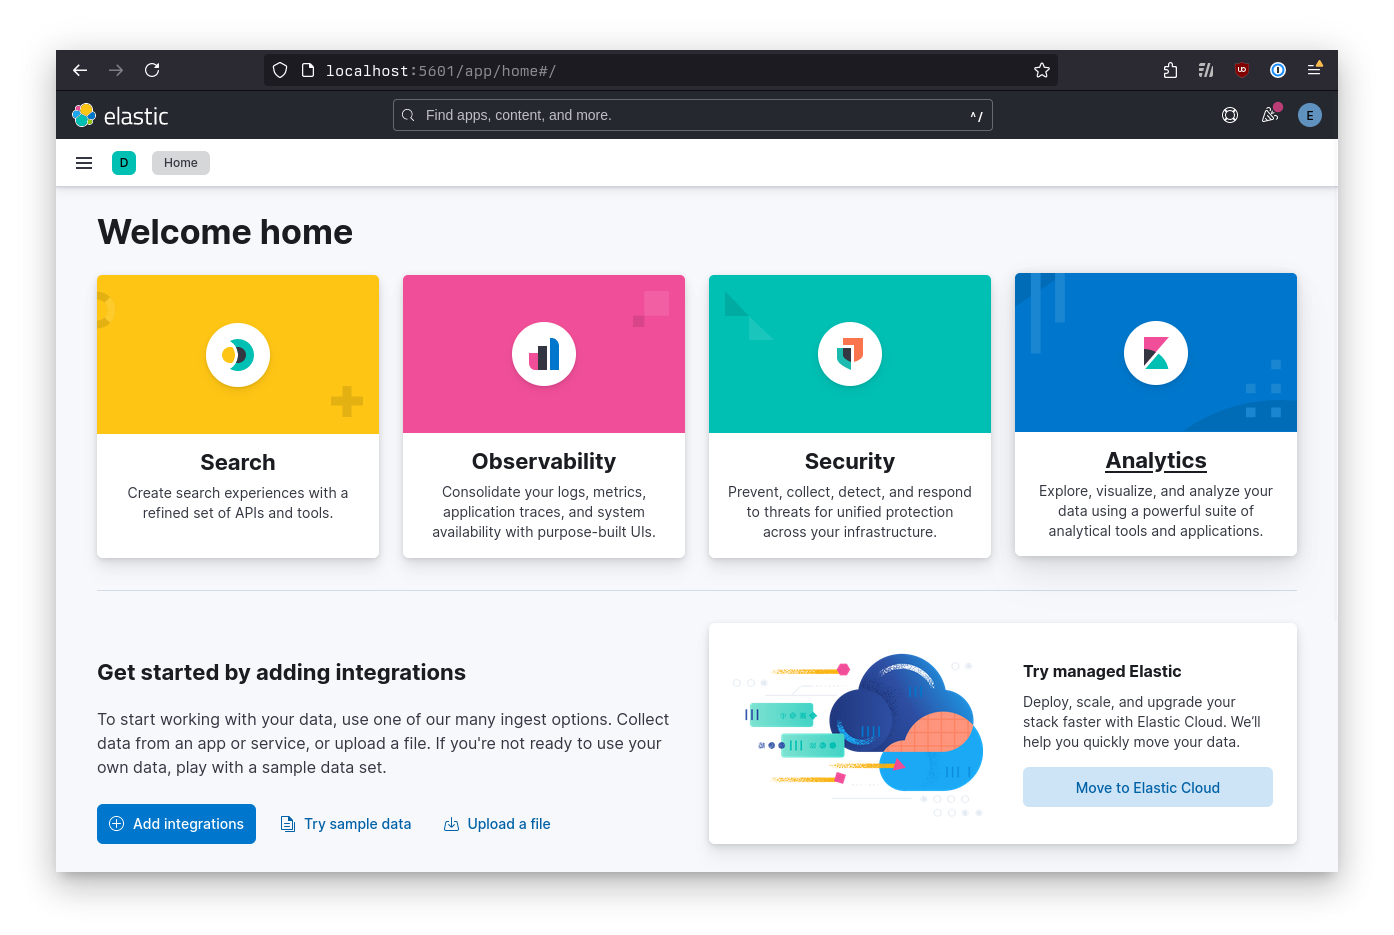
\includegraphics[width=\textwidth]{impl/local2.png}
	\caption{Página de inicio de Kibana}
	\label{fig:kibana_start}
\end{figure}

Una vez aquí, se puede hacer click en la opción \texttt{Try sample data} para
cargar un conjunto de datos de ejemplo y probar la funcionalidad de Kibana con
Elasticsearch. Por supuesto, también se pueden probar la ingesta de datos a
través de Logstash y Kafka o, si así se desea, a través de los \textit{Beats}
especializados de ingesta directa de Elastic.

El código de despliegue local se encuentra en \fullref{anexo:local}. El
manual de uso del sistema se encuentra en \fullref{sec:manual_usuario}.


\newpage{}
\section{Despliegue \textit{cloud}}\label{sec:impl_cloud}
El desarrollo principal del despliegue en la nube se concentra en la creación
de los scripts de \textit{Terraform} necesarios para la implementación de la
infraestructura planteada en el apartado \fullref{sec:arquitectura}. Para ello,
se divide el proyecto en scripts separados de manera que se puedan gestionar
los recursos y los servicios de manera independiente.

El diseño de una infraestructura base y el desarrollo de un prototipo de manera
local permiten tener una idea clara de los recursos necesarios y de las
características específicas de cada servicio, facilitándo la tarea de
desarrollo.

% TODO: desarrollar

Para el desarollo, se hace uso de un repositorio privado en \textit{Bitbucket}
para el control de versiones y facilitar a la empresa la revisión y uso del
código.



\newpage{}
\section{Ingesta de datos}\label{sec:impl_ingesta}
Tras la creación y el despliegue de la infraestructura base, se procede a la
creación de los scripts de ingesta de datos, de manera escalonada y siguiendo
la prioridad de las fuentes de datos.

Puesto que se ha decidido utilizar Kafka como sistema de mensajería, se
desarrollan los scripts de ingesta de datos para que los datos se envíen a
Kafka y se procesen mediante Logstash y Elasticsearch.

Para la ingesta de datos, se han desarrollado scripts de Python que se encargan
de la lectura de los datos de las fuentes, su transformación y su envío a Kafka.
Estos scripts se ejecutan mediante un \textit{cron} que se encarga de la
ejecución periódica de los mismos.


\newpage{}
\section{Visualización de datos}\label{sec:impl_visualizacion}
Una vez se cuentan con datos en Elasticsearch, se puede comenzar el desarrollo
de la visualización de los mismos mediante Kibana. Para ello, se han desarrollado
paneles de visualización que permiten la monitorización de los datos en tiempo
real y la creación de informes y \textit{dashboards} personalizados para cada
modelo de datos contemplado.
